%%% Fiktivní kapitola s ukázkami citací

\chapter{Definice požadavků}\label{chap:requirements}

Abychom navrhli a~implementovali v~praxi použitelný systém, musíme nejprve podrobněji rozebrat, jaké požadavky jsou na systém kladeny. 

\section{Funkční požadavky}

Jednotlivé funkční požadavky si představíme ve formě uživatelských příběhů (anglicky \textit{user stories}).
Jak uvádí Fred Health, jedná se o~formu zaznamenávání funkčních požadavků na systém ve strukturované podobě krátkých příběhů většinou vypadajících následovně: 

„Jako \textit{typ uživatele} chci, nebo potřebuji \textit{nějakou funcionalitu}, aby \textit{nějaký benefit}.“\cite{userStories}  

Tato forma zápisu nám pomůže konzistentně strukturovat informace o~tom, jakou funkcionalitu potřebuje jaký typ uživatele a~proč ji daný typ uživatele potřebuje, což zužitkujeme při tvorbě designu systému (viz kapitola \ref{chap:design}).

Definujeme si 2 typy uživatelů systému:

\begin{itemize}
    \item Zákazník — je uživatel využívající systém pro mapování a~vizualizaci dat.
    \item Správce systému — je zaměstnanec provozovatele systému, který má na starost správu zákazníků a~poskytování asistence s~jejich problémy.
\end{itemize}

Dále si upřesníme některé pojmy, jež budeme v~příbězích užívat:

\begin{itemize}
    \item Nový zákazník — je zákazník, s~nímž byla nově domluvena spolupráce a~ještě pro něj není vytvořený uživatelský účet.
    \item Stávající zákazník — je zákazník, pro něhož je vytvořený účet a~může používat všechny části systému, tzn. již pro něj je dostupná instance nástroje \textit{Metabase}. 
    \item Bývalý zákazník — je zákazník, s~nímž byla spolupráce rozvázána.
    \item Mapování dat — je dle Wikipedie proces vytváření mapování mezi elementy dvou datových modelů, např. za účelem pozdější tranformace dat mezi danými datovými modely\cite{dataMapping:online}.
    My se omezíme na mapování mezi relačními modely.
    
    \item Generický datový model — je datový model, který je dostatečně zobecněný, abychom na něj mohli převést, v našem případě, data od různých zákazníků.
    \item Mapovací nástroj — je jeden z~modulů našeho systému, který umožňuje zákazníkům mapovat data na generický datový model systému.
    \item Mapovací projekt — označení pro mapování dat jednoho zákazníka na generický datový model systému.
    \item Klastr — pojemem klastr (anlgicky \textit{cluster}) je myšlen Kubernetes klastr\footnote{Více informací v podsekci \ref{subsec:k8s}.}.
    \item Dashboard - je dle Wikipedie typ grafického UI, který umožňuje jednoduše na jednom místě sledovat hlavní ukazatele výkonnosti\footnotemark{} dané organizace ve strukturované podobě \cite{Dashboards:online}.
    V našem případě se bude jednat o~dashboardy z nástroje \textit{Metabase}.
\end{itemize}
\footnotetext{Více na \url{https://en.wikipedia.org/wiki/Performance_indicator}.}

Uživatelské příběhy rozdělíme do dvou následujících podsekcí podle typu uživatele.



\subsection{Příběhy správce systému}

\begin{enumerate}
    \item Jako správce systému potřebuji přidávat \textit{nové zákazníky}, aby mohli začít používat systém.
    \item Jako správce systému potřebuji mazat \textit{bývalé zákazníky}, aby jen \textit{stávající zákazníci} měli přístup do systému.
    \item Jako správce systému potřebuji nahlížet do \textit{mapovacích projektů} zákazníků, abych mohl poskytnout asistenci s mapováním nebo mohl provést kontrolu \textit{mapování}.
    \item Jako správce systému potřebuji zajistit spuštění nové instance nástroje \textit{Metabase} v \textit{klastru}, aby jej zákazník  mohl začít používat.
    \item Jako správce systému potřebuji, aby systém v případě spuštění nové instance nástroje \textit{Metabase} automaticky provedl zpracování mapování a zpřístupnil vizualizaci dat daného zákazníka pomocí nové instance.
    \item Jako správce systému potřebuji, aby systém vyžadoval přihlášení po všech uživatelích, aby uživatelská data nebyla zpřístupněna neoprávněným osobám.
    \item Jako správce systému v případě, kdy zákazník odejde od \textit{Firmy}, potřebuji, aby systém ukončil instanci nástroje \textit{Metabase} příslušící danému uživateli, aby jej již nemohl používat.
    
\end{enumerate}

Příběhy správce jsou shrnuty formou use case diagramu\footnote{
Diagram případů užití (anglicky \textit{use case diagram}) je v softwarovém inženýrství jeden z~UML diagramů chování \cite{useCaseDiagWiki:online}.
}
na obrázku \ref{fig:admin-use-cases}.
\begin{figure}
    \centering
    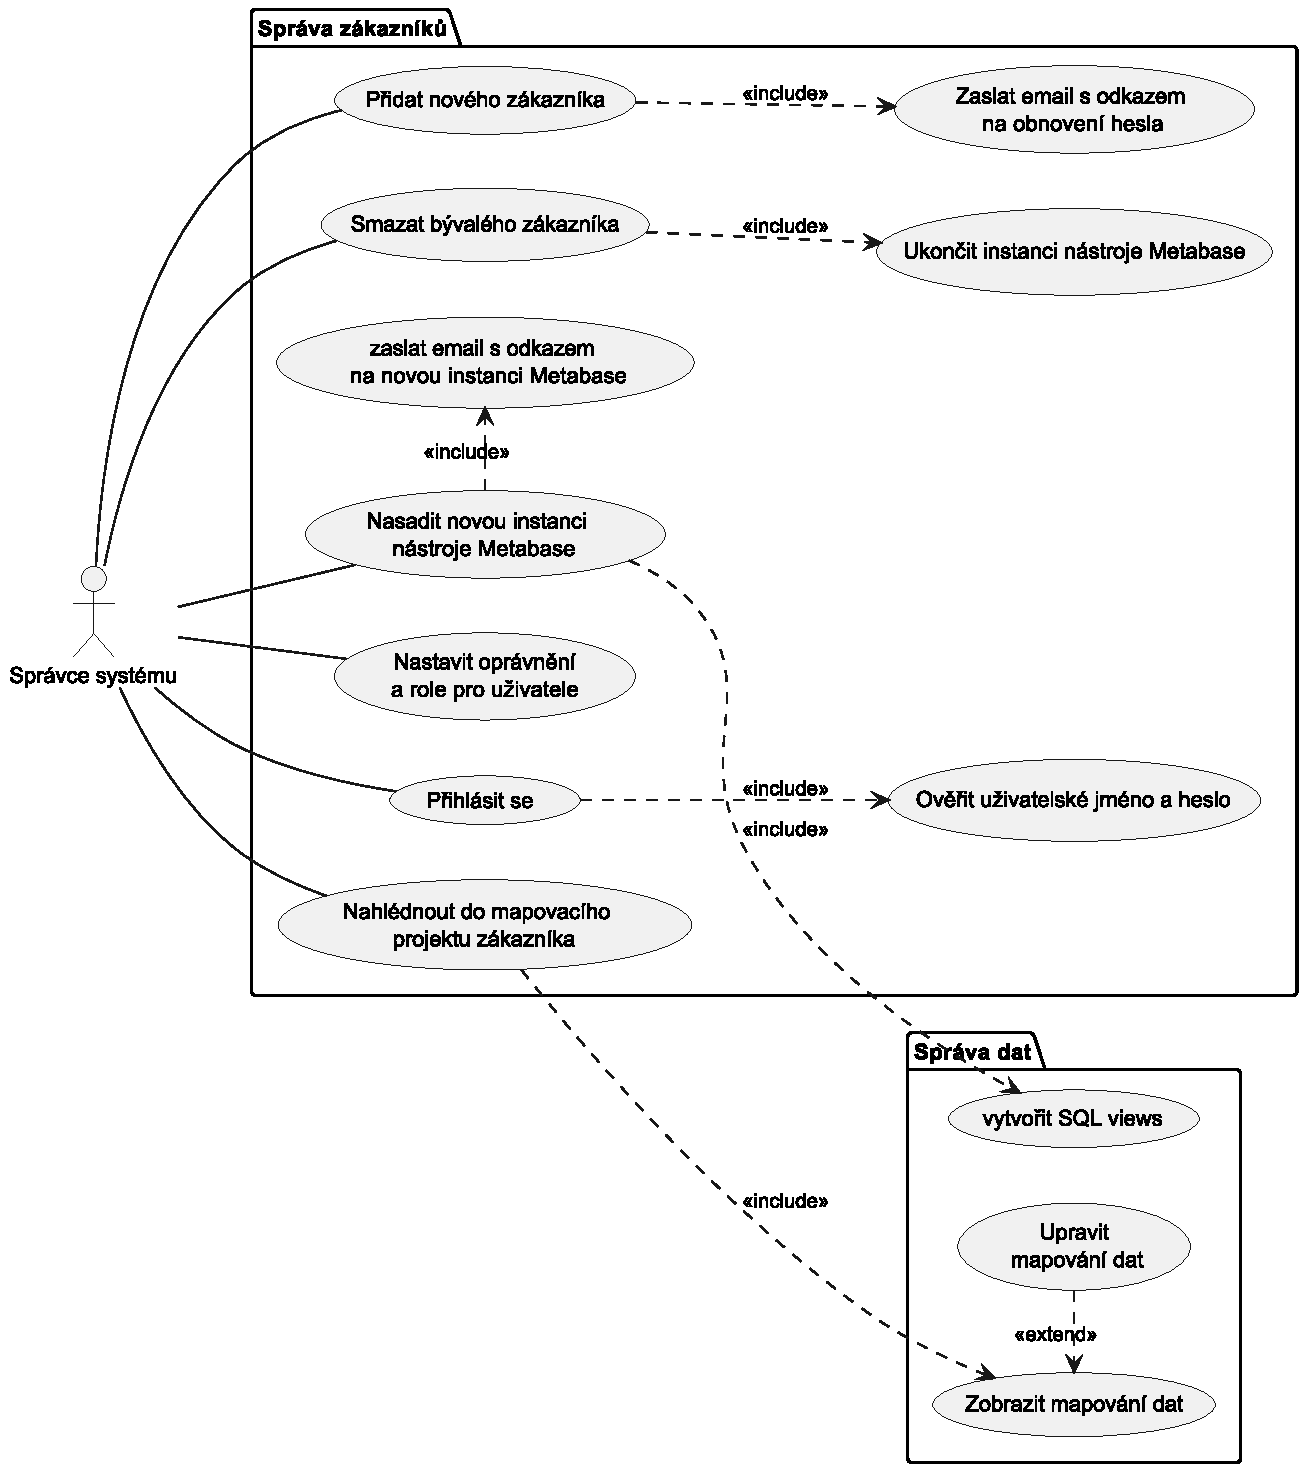
\includegraphics[width=\linewidth]{img/Use Case Diagram - Správce systému (1).pdf}
    \caption{Diagram případů užití systému správcem}
    \label{fig:admin-use-cases}
\end{figure}

\subsection{Zákaznické příběhy}

\begin{enumerate}
    \item Jako zákazník potřebuji připojit svoji Microsoft SQL Server\footnote{Více na \url{https://www.microsoft.com/cs-cz/sql-server}} databázi ERP systému k systému, abych mohl začít mapovat svoje data na \textit{generický datový model}.
    \item Jako zákazník potřebuji používat uživatelsky přívětivý \textit{nástroj pro mapování dat}, abych mohl snadno a~rychle převést svoje data na generický datový model.
    \item Jako zákazník potřebuji mít možnost zadat přístupové ke své databázi, aby systém mohl připravit mapování dat.
    \item Jako zákazník potřebuji mít možnost upravovat nebo změnit mapování dat, abych mohl reagovat na změny v~mých datech nebo požadavcích.
    \item Jako zákazník potřebuji mít přístup k nástroji \textit{Metabase}, abych mohl vizualizovat a~analyzovat svoje data pomocí různých reportů a dashboardů.
    \item Jako zákazník potřebuji mít možnost sdílet nebo exportovat svoje reporty a~dashboardy, abych mohl prezentovat nebo sdílet svoje výsledky s~ostatními.
    \item Jako zákazník potřebuji mít možnost poskytnout zpětnou vazbu nebo požádat o~podporu, abych mohl řešit případné problémy nebo potřeby v rámci systému.
\end{enumerate}

Výše uvedené požadavky zjednodušeně ilustruje use case diagram \ref{fig:customer-use-cases}.

\begin{figure}
    \centering
    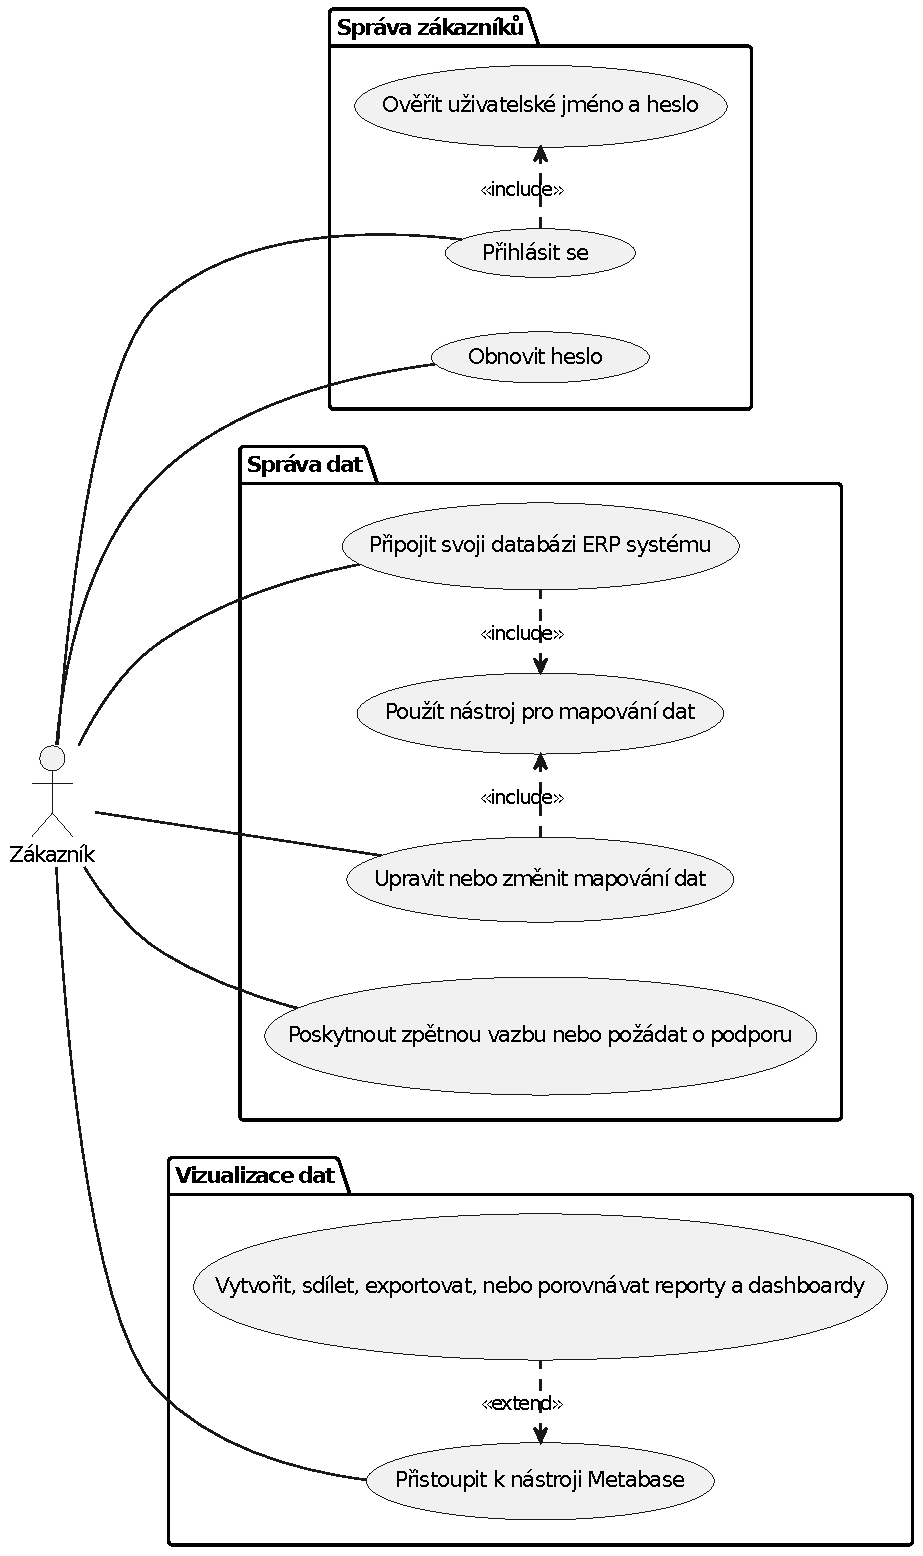
\includegraphics[width=0.75\linewidth]{img/Use Case diagram - Zákazník (2).pdf}
    \caption{Diagram případů užití systému zákazníkem}
    \label{fig:customer-use-cases}
\end{figure}


\section{Nefunkční požadavky}

Podle Sommervilla jsou nefunkční požadavky\footnote{Z anglického \textit{non-functional requirements}.} omezení kladená na systém jako celek spíše než požadavky na jednotlivé funkce systému.
Sommerville dále uvádí, že tyto požadavky jsou mnohdy zásadnější než mnohé funkční požadavky \cite{Sommerville}(strana 85-88), tudíž i~my si patřičně rozebereme, jaké nefunkční požadavky musí námi vyvíjený systém splňovat.

Typů nefunkčních požadavků existuje celá řada~\cite{NonFunct69:online}, jak ilustruje obrázek \ref{fig:non-func-types}. My se tudíž v~následujících podsekcích zaměříme jen na několik hlavních.

\begin{figure}
    \centering
    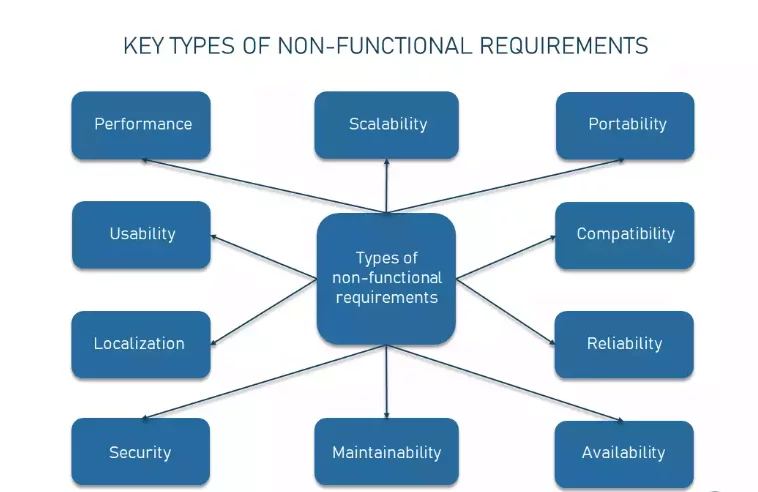
\includegraphics[width=0.75\linewidth]{non-functional-req-types.png}
    \caption{Základní typy nefunkčních požadavků, zdroj: Testomat.io, 2023, dostupné z~\url{https://testomat.io/wp-content/uploads/2023/03/Key_Software_Req.png}}
    \label{fig:non-func-types}
\end{figure}

\subsection{Výkonnost}
Jelikož se neočekává, že systém budou využívat stovky či tisíce uživatelů současně, požadavky na výkon jsou zaměřeny spíše na náročnější akce, které by měl systém vykonávat.

\begin{itemize}
    \item Nasazení nové instance nástroje Metabase nesmí trvat déle než 30 sekund.
    \item Vytvoření nového projektu zákazníka nesmí trvat déle než 30 sekund.
\end{itemize}

\subsection{Použitelnost}

Tento aspekt systému je zejména z pohledu zákazníka klíčový.
Konfigurace přístupových údajů k zákaznické databázi a mapování dat musí být co nejintuitivnější. 70~\% zákazníků musí tento proces zvládnout samostatně.

\subsection{Udržitelnost}

Systém musí být rozdělen do modulů a komponent, aby se snížila nutnost zasahovat do různých částí systému v případě změny v pouze určité části.

\subsection{Bezpečnost}

Jelikož pracujeme se zákaznickými daty, je naprosto zásadní, aby tato data zůstala chráněna.

\begin{itemize}
    \item Všichni uživatelé musí být autentizováni.
    \item Přístupové údaje daného zákazníka si může zobrazit a~modifikovat pouze daný zákazník.
    \item Zákazníci nesmí být schopni si navzájem nahlížet do mapování dat. 
\end{itemize}

\subsection{Interoperabilita}
\begin{itemize}
    \item Systém musí pro export mapování využívat formát JSON.
    \item Systém musí podporovat databázový systém \textit{Microsoft SQL Server} a být připraven na rozšíření podpory pro další databázové systémy.
\end{itemize}

\subsection{Škálovatelnost}

Systém musí být schopný provozovat 30 instancí nástroje \textit{Metabase} zároveň.

\subsection{Portabilita}

Systém musí podporovat jakoukoliv platformu, která umožňuje běh Docker kontejnerů\footnote{Více informací na \url{https://cs.wikipedia.org/wiki/Docker}.}.

\subsection{Testovatelnost}

Systém musí být obohacen o testovací data a testovací prostředí, které umožní běh celého systému pro integrační testování.
Kód systému musí využívat programovací techniky enkapsulace\footnote{Více informací na \url{https://en.wikipedia.org/wiki/Encapsulation_(computer_programming)}} pro usnadnění testování jednotlivých komponent.